%If you have a single appendix, you need to change {\chapter*{APPENDIX: THIS IS THE FIRST APPENDIX}
%to {\chapter*{APPENDIX: YOUR APPENDIX TITLE HERE} if you have two or more appendices
%you need to change {\chapter{THIS IS THE FIRST APPENDIX}} to
%{\chapter{YOUR APPENDIX TITLE HERE}}
%
%If you make these changes correctly Latex will complain bitterly about the additions to the TOC
%but will make them correctly in a manner acceptable to the Editorial Office.

%\ifthenelse{\value{noa} = 1}
%...................then
%{\chapter*{APPENDIX: STRUCTURED OVERLAY BROADCAST}
%\label{broadcast}
%\addcontentsline{toc}{chapter}{APPENDIX: STRUCTURED OVERLAY BROADCAST}
%\chaptermark{Appendix}
%\markboth{Appendix}{Appendix}
%\setcounter{chapter}{1}}
%...................else
{\chapter{STRUCTURED OVERLAY BROADCAST}
\label{broadcast}}
%...................


Brunet has an efficient broadcast model called bounded-broadcast because it is
capable of broadcasting to a subset of nodes, though it is also capable of
broadcasting to the entire overlay.  A bounded broadcast uses the following
recursive algorithm:  Begin with node $x$ triggering a broadcast message over
the region $[x, y]$.  $x$ has $F$ connections to nodes in the range $[x, y]$.
Denoting the $i^{th}$ such neighbor as $b_i$, the node $x$ sends a bounded
broadcast over a sub-range, $[b_i, b_{i+1})$, to $b_i$, except the final
neighbor.  Differently stated, $b_i$ is in charge of bounded-broadcasting 
in the sub-range $[b_i, b_{i+1})$. If there is no connection to a node in the
sub-range, the recursion has ended.  The final neighbor, ($b_F$), is responsible
for continuing the bounded broadcast from $[b_F, y]$.  When a node receives a
message to a range that contains its own address the message is delivered to
that node and then routed to others in that range.  Figure \ref{fig:tree} shows
how this bounded broadcast forms a local tree recursively.   The time required
for a bounded broadcast is $O(\log^2 N)$ as shown in~\cite{small_world}.  To
perform a broadcast on the entire overlay, a peer performs the bounded-broadcast
starting from its node ID with the end address being the node ID immediately
preceding its own in the address space.  

\begin{figure}[ht]
\centering
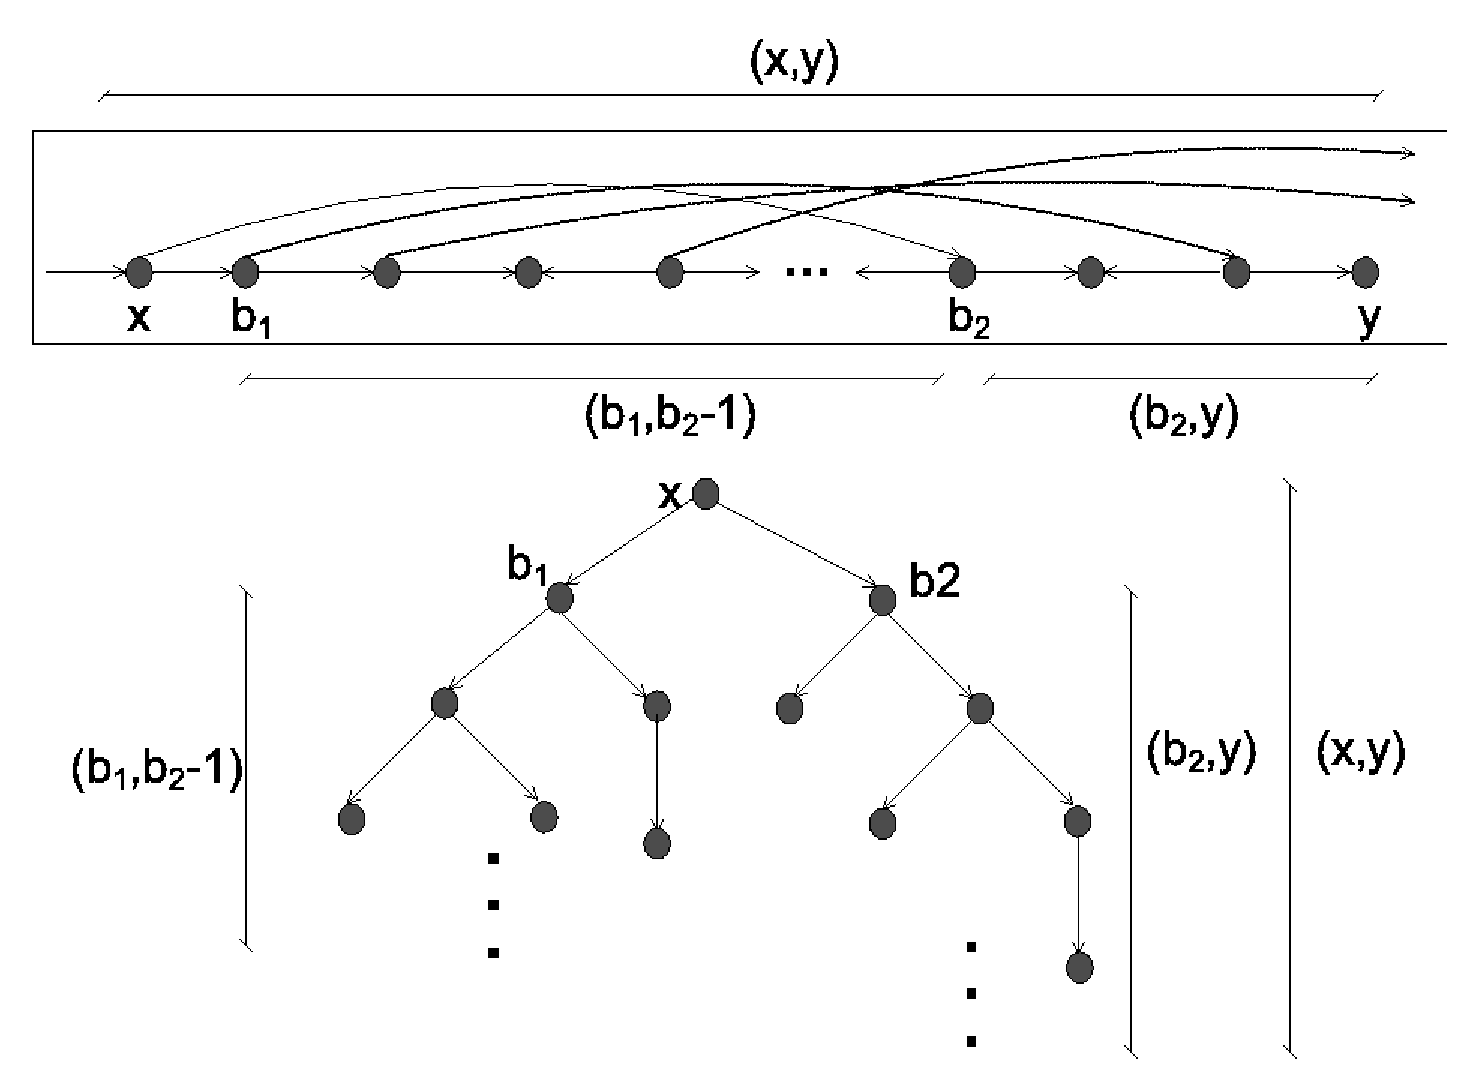
\includegraphics[width=4in]{tree.eps}
\caption{Bounded Broadcast in range $[x, y]$}
\label{fig:tree}
\end{figure}
